\begin{frame}{Introduction}
	\vfill
	\begin{quotation}
		\centering
		Game theory is the mathematical study of interaction\\
		among independent, self-interested agents.\\
		{\color{colornote}-- Essentials of Game Theory, \cite{leyton2008essentials}}
	\end{quotation}

	\vfill
	\textbf{Examples}: economic and ecological games, machine learning, etc. \textcolor{colornote}{$\rightsquigarrow$ \emph{cybernetics}.}

	\vfill
	% ugh
	\onslide<2->{
		\alt<3>{
			Open games as a framework for compositional game theory

			\begin{center}
				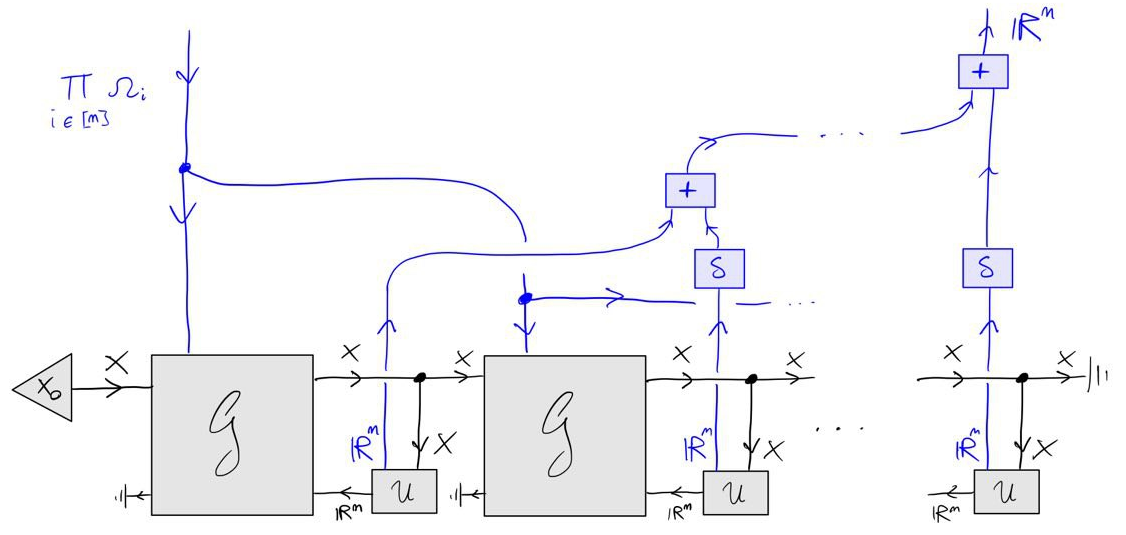
\includegraphics[width=.8\textwidth]{figures/og_ex.png}
			\end{center}

			Shows causality without being too unwieldy, compositional (\textcolor{coloraccent}{$\rightsquigarrow$ large scale}).\\
			Also: string diagrams are nice to work with!
		}{
			Classical game theory: \textbf{normal form} and \textbf{extensive form}

			\begin{center}
				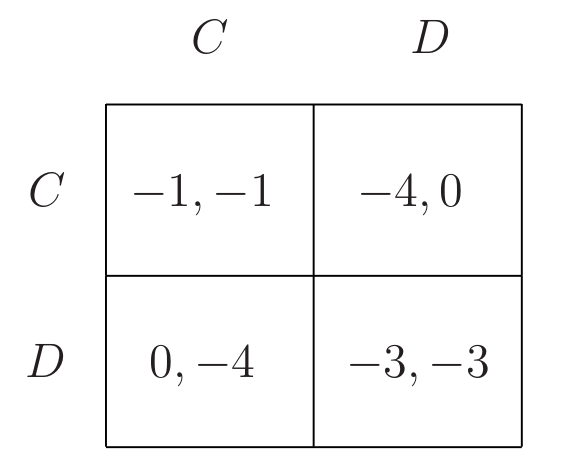
\includegraphics[width=.34\textwidth]{figures/pd_norm.png}
				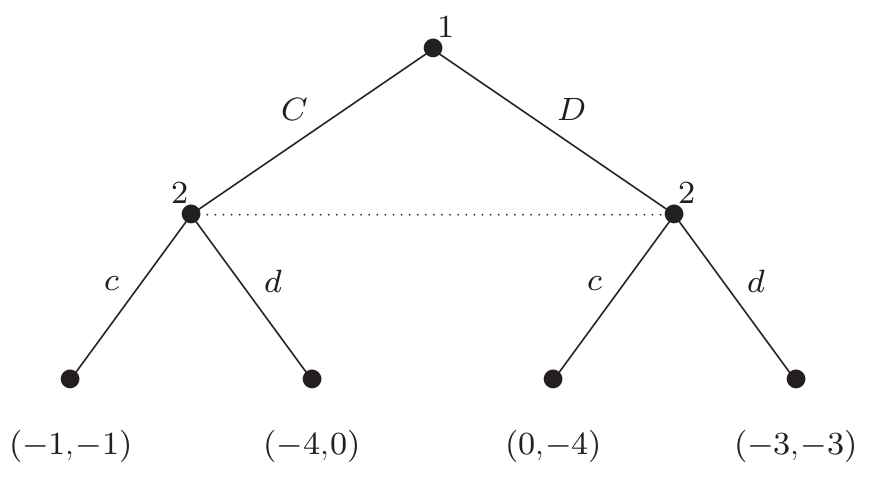
\includegraphics[width=.5\textwidth]{figures/pd_ext.png}
			\end{center}

			\textbf{Drawbacks}: too little information (NF), too much information (EF), unclear causal relationships (both). Most importantly: non-compositional! (\textcolor{coloraccent}{$\rightsquigarrow$ small scale})
		}
	}
\end{frame}

\begin{frame}{Introduction}
	Translating NF to open games is 'trivial' (there's only a utility function)...

	\begin{center}
		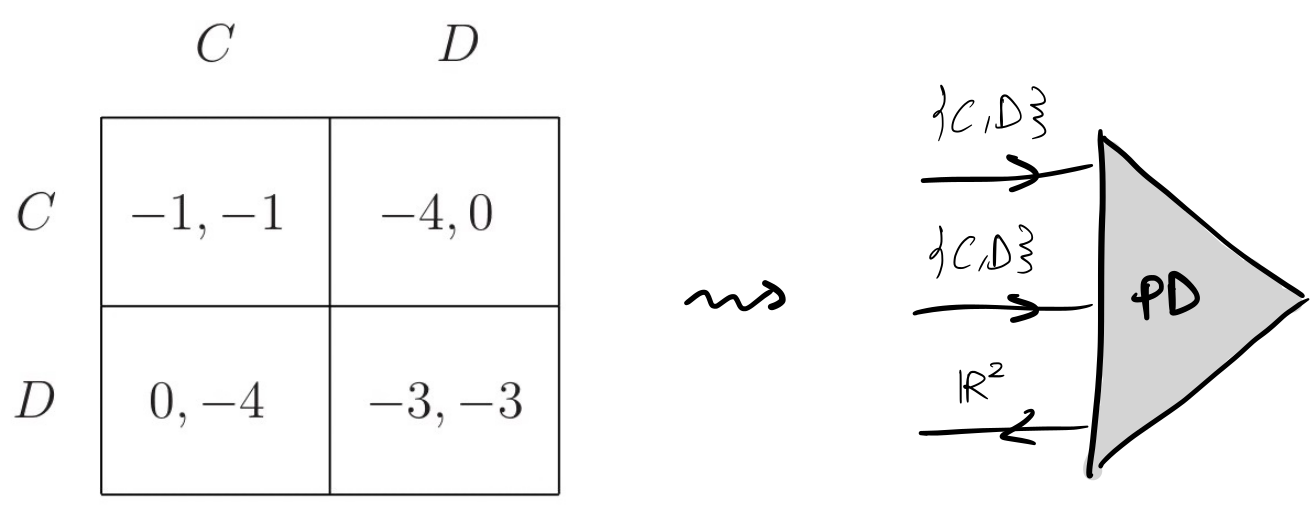
\includegraphics[width=.7\textwidth]{figures/nf_to_og.png}
	\end{center}

	\onslide<2->{
		Translating EF to open games (mantaining a similar causal structure) is non-trivial:
		\begin{enumerate}
			\item EF is a \textbf{non-inductive definition}, and it's messy to map a whole tree in one go.
			\item Open games don't have an \textbf{explicit notion of players}, necessary to model imperfect information and to correctly compute equilibria.
		\end{enumerate}
	}
	\onslide<3->{
		To do so, we introduce:

		\begin{enumerate}
			\item Open games with \textbf{agency}, an improved compositional framework for games,
			\item An operator calculus for games, in particular new \textbf{choice operators},
			\item \textbf{Inductive data types for EF trees} with (im)perfect information.
		\end{enumerate}
	}
\end{frame}

% 1. Open Games with Agency
% - lenses and bidirectional information flow (= attuale)
% - straight to: arena as parametrised lens (slide 12 ma con strat (slide 23 but rename costrategies and redraw))
% - composition
% - choice
% - reparametrisation & regrouping
% - closing an arena: state and payoff
% - keep slide 18
% - keep slide 22-25 but (a) condense intro to 1 slide, (b) slide 25 on directly exemplify lens_S (or not?)
% - slide 27 add '\in \varepsilon \boxtimes \eta(k)' to the diagram
% - put slide 28 in slide 29 with def

% 2. Extensive form and translation
% - lots of pictures of trees
% - PETree & defs
% - translation: a single picture
% - an example (probably to work out 'live'?)
% - IETree & defs
% - translation: a single picture
% - an example (probably to work out 'live'?)

% 3. Future work
% - Functoriality?
% - Copy from paper
